\documentclass{ximera}
\graphicspath{{./content/hw_04_arclength_curvature/graphics/}{./graphics/}}
\title{Homework 4: Arclength and Curvature}
\begin{document}
\begin{abstract}
\end{abstract}
\maketitle

SOME PROBLEMS COPIED FROM HANDOUTS - NOT SURE OF THEIR SOURCE

\section*{Online Problems/Completion Packet}

\begin{problem}
Compute the length of the path $\vec{x}(t)=\left(2,t^2,\frac{1}{3}t^3\right)$ for $-2\leq t\leq 2$.
\end{problem}

\begin{problem}
Compute the length of the path $\vec{x}(t) = \left(t, 4\sqrt{t}, 2\ln(t)\right)$ for $1\leq t\leq 4$.
\end{problem}

\begin{problem}
In single variable calculus, you learned the formula $L=\int_a^b\sqrt{1+(f'(x))2}dx$ for the length of the curve defined by $y=f(x)$ for $a\leq x\leq b$. In this problem, you will show that our new definition for arclength coincides with this single variable formula.

The curve $y=f(x)$, for $a\leq x\leq b$, can be parametrized as $\vec{x}(t) = (t,f(t))$ for $a\leq t\leq b$. Prove that the the length of $\vec{x}(t)$ is $\int_a^b\sqrt{1+(f'(x))2}dx$.
\end{problem}

\begin{problem}
Consider the path
\[
\vec{x}(t) = \begin{cases}
(t,0) & 0\leq t\leq 1\\
(1,t-1) & 1\leq t\leq 2\\
(3-t, 1) & 2\leq t\leq 3\\
(0, 4-t) & 3\leq t\leq 4
\end{cases}.
\]
\begin{enumerate}
\item Sketch this path.
\item Is this path $C^1$? Explain.
\item Find the length of the path.
\end{enumerate}
\end{problem}

\begin{problem}
Consider the path $\vec{x}(t) = \left(\frac{\cos(t)}{t^2},\frac{\sin(t)}{t^2}\right)$ for $t\in [1,\infty)$.
\begin{enumerate}
\item Sketch this path.
\item Compute $\int_1^\infty\|\vec{x}'(t)\|\;dt$.
\item Explain why we consider this path to have finite length, even though the parameter is unbounded.
\end{enumerate}
\end{problem}

\begin{problem}
%copied from handout
Find the curvature of $\mathbf{x}(t)=(t,t^{2},t^{3})$ at the point $(1,1,1)$.
\end{problem}

\begin{problem}
%copied from handout
Consider the curve $C$ shown below.
\begin{image}
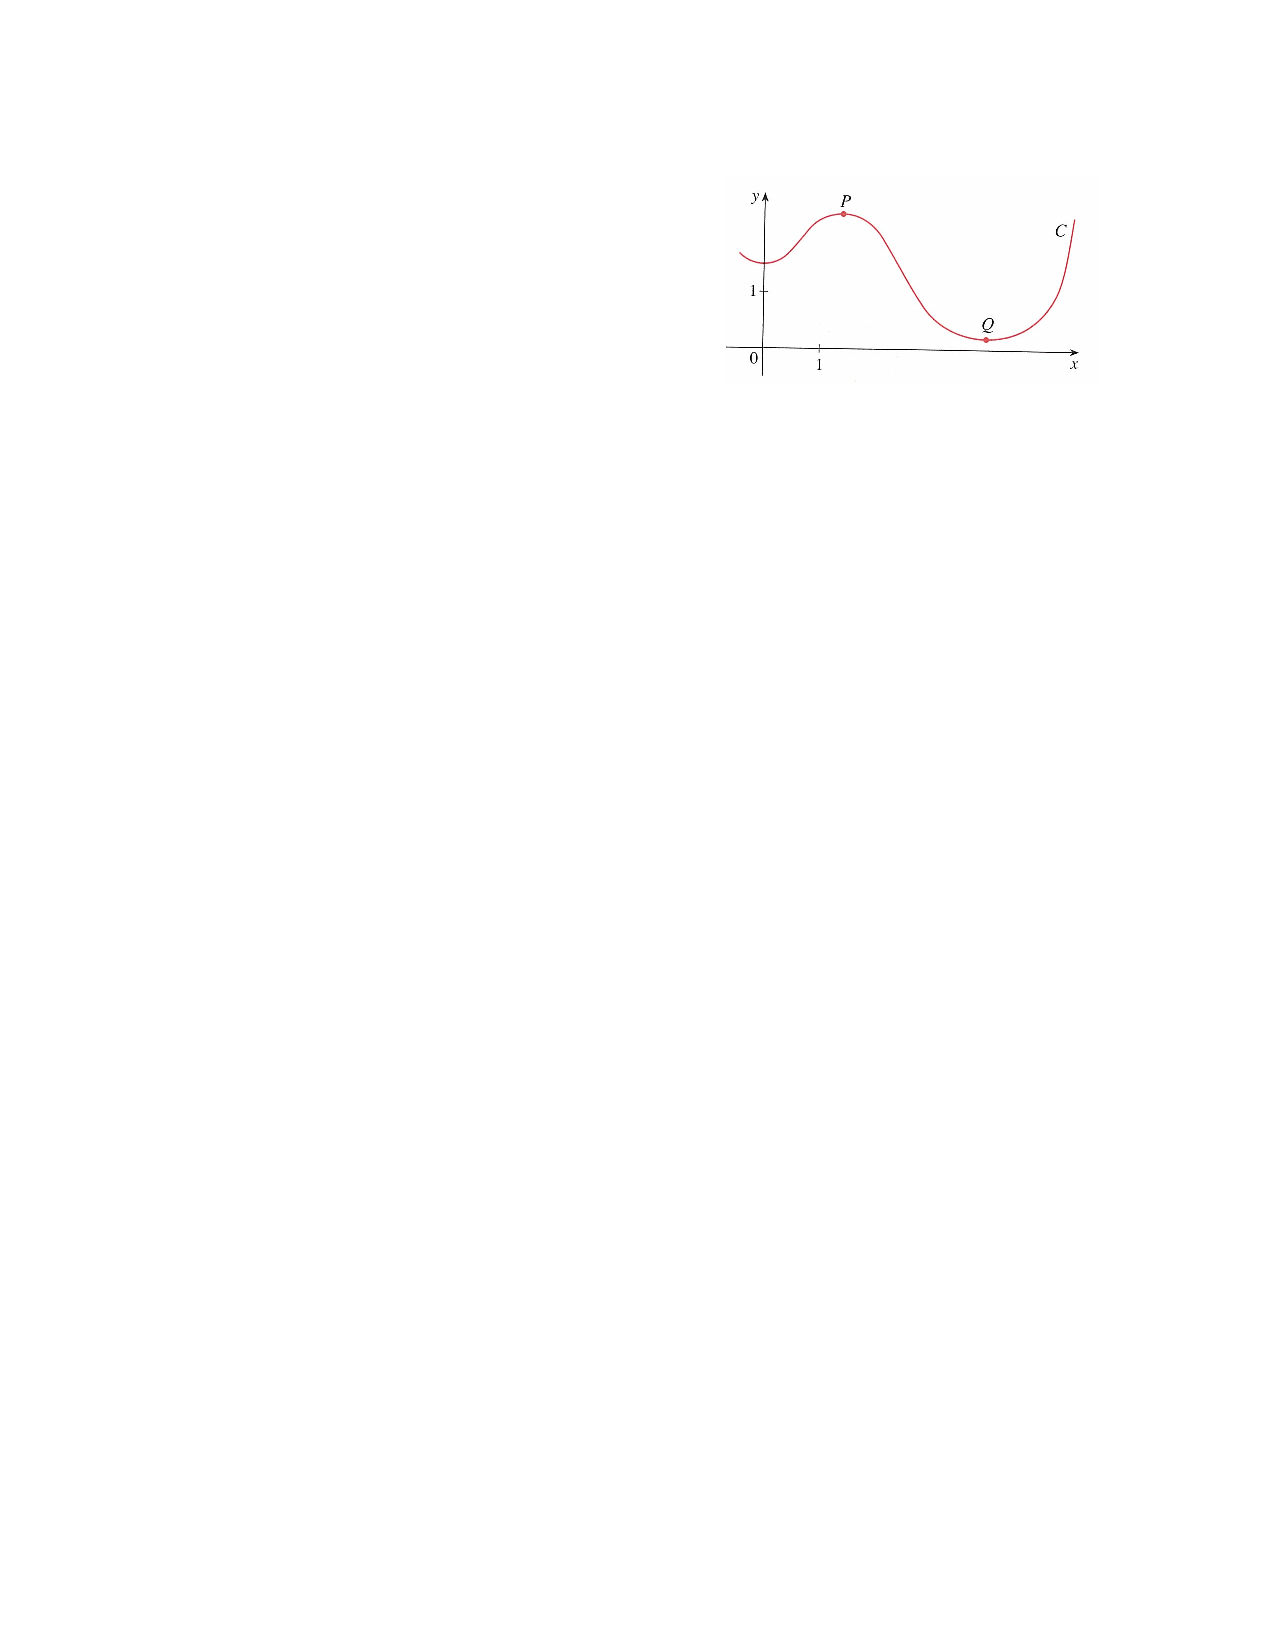
\includegraphics[width = \textwidth]{curvyCurve}
\end{image}
\begin{enumerate}
\item Is the curvature of the curve $C$ greater at $P$ or at $Q$?  Explain.
\item Estimate the curvature at $P$ and at $Q$ by sketching the osculating circles at those points.
\end{enumerate}
\end{problem}

\begin{problem}
%copied from handout
Each of the graphs below has two curves, $a$ and $b$.  In each case one of the curves is a graph of the curvature of the other.  Identify which is the original curve and which is the graph of the curvature.  Explain your answers
\begin{image}
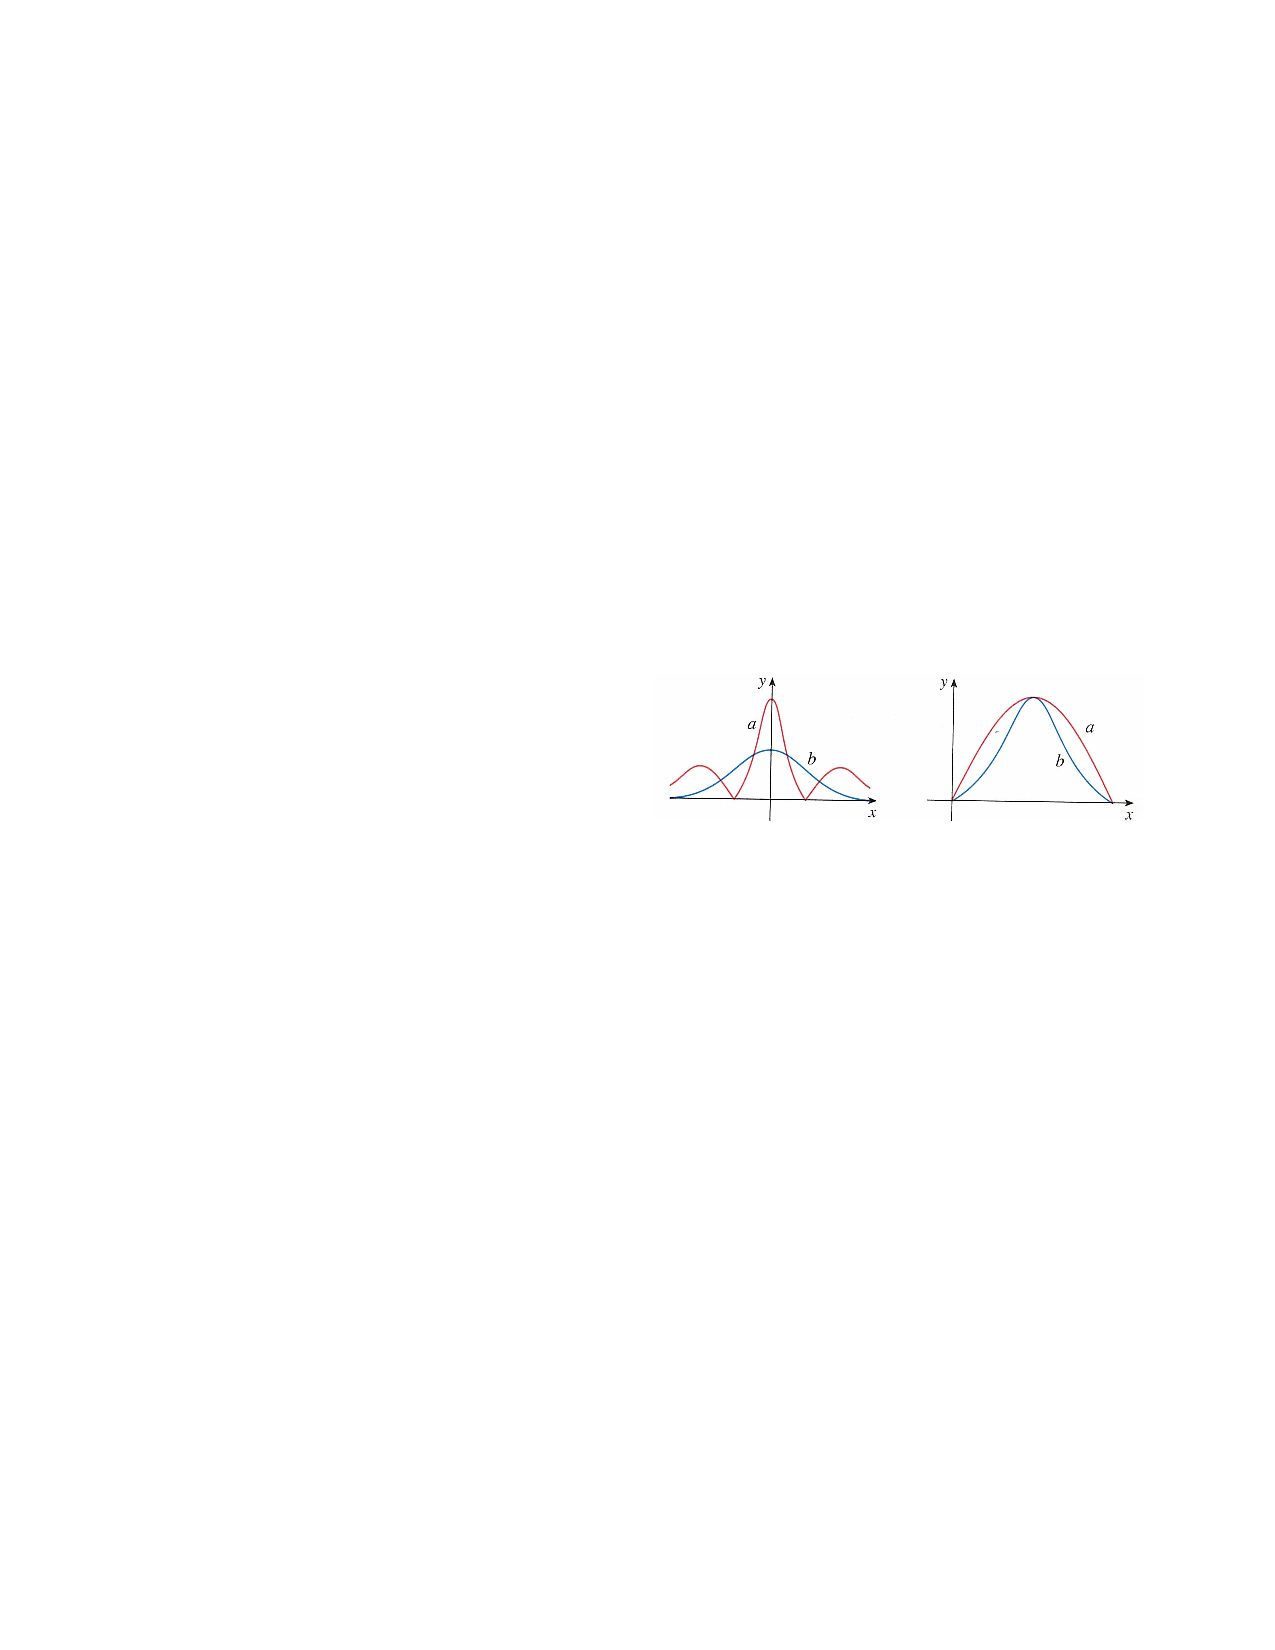
\includegraphics[width = \textwidth]{curvatures}
\end{image}
\end{problem}

\begin{problem}
%copied from handout
Find an equation of a parabola that has curvature 4 at the origin.  Use the definition of curvature given in class.  Make sure to justify your answer with pictures, calculations, and other explanations.  Hint: it will help to simplify your calculations at each point.  For example, $\mathbf{T}'(t)$ and $\mathbf{T}'(t) \cdot \mathbf{T}'(t)$ may appear messy, but can be greatly simplified.
\end{problem}

\section*{Written Problems}

\begin{problem}
Compute the length of the path $\vec{x}(t) = (2t^3,3t^2)$ for $0\leq t\leq 5$.
\end{problem}

\begin{problem}
%copied from handout
\begin{enumerate}
\item Parametrize the graph of $y = \ln x$.  At what point does the curve have maximum curvature?  What happens to the curvature as $x \to \infty$?
\item Parametrize the graph of $y = e^{x}$. \emph{Without calculating $\kappa(t)$, answer these questions:} At what point does the curve have maximum curvature?  What happens to the curvature as $x \to \infty$? (Hint: Use the geometric relationship between the functions in parts a and b.) %Too easy with this hint?
\end{enumerate}
\end{problem}

\section*{Professional Problem}

\begin{problem}
%copied from handout, reworked for online format (handout had space for solution).
In this problem you will prove that the value of the integral used to compute arclength is independent of parametrization.  First prove the following version of the chain rule, which will be needed later.  Your proof will be evaluated as part of your solution to the professional problem.
\begin{proposition}
Let $\vec{x}:I \to \mathbb{R}^n$ be a smooth path, and $f(t)$ a differentiable function from $\mathbb{R}$ to $\mathbb{R}$.  Then 
\[ \frac{d}{dt} \vec{x}\left( f(t) \right) = \vec{x}'\left( f(t) \right) f'(t). \]
\end{proposition}

Next, prove the following theorem.

\begin{theorem}
Let $\vec{x}: [a,b] \to C$ and
$\vec{y}: [c,d] \to C$
be two smooth and simple (that is, not self-intersecting) parametrizations of a curve $C$ in $\mathbb{R}^n$ with the same starting and ending points,  so $\vec{x}(a)=\vec{y}(c)$ and $\vec{x}(b)=\vec{y}(d)$.  Then
\[ \int_a^b || \mathbf{x}'(t) || \, dt = \int_c^d || \mathbf{y}'(s) || \, ds. \]
\end{theorem}

\textit{Hints:
\begin{itemize}
\item Define a new function, $f(t) = \vec{y}^{-1} \left( \vec{x}(t) \right)$.
\item Write out the arclength integral in terms of $\vec{x}$, rewrite $\vec{x}(t)$ as $\vec{y}\left( f(t) \right)$, and use the above proposition and $u$-substitution to transform the left side into the right side.
\item $\vec{y}^{-1}$ exists, so the definition for $f$ makes sense. (You'll need to justify this statement.)
\item $f:[a,b] \to [c,d]$, $f(a) = c$ and $f(b)=d$. (You'll need to justify this statement.)
\item $f$ is strictly increasing. (You'll need to justify this statement.)
\item $\vec{x}(t) = \vec{y}\left( f(t) \right)$. (You'll need to justify this statement.)
\end{itemize}
}

\end{problem}



\end{document}